\documentclass{beamer}
%\usepackage[utf8]{inputenc}
%\usetheme{Warsaw}
\usetheme{CambridgeUS}
%\usecolortheme{seahorse}

%-------------------------------------------------------------------------------
%          -Packages nécessaires pour écrire en Français et en UTF8-
%-------------------------------------------------------------------------------
\usepackage[utf8]{inputenc}
\usepackage[frenchb]{babel}
\usepackage[T1]{fontenc}
\usepackage{lmodern}
\usepackage{textcomp}

%-------------------------------------------------------------------------------

%-------------------------------------------------------------------------------
%                          -Outils de mise en forme-
%-------------------------------------------------------------------------------
\usepackage{hyperref}
\hypersetup{pdfstartview=XYZ}
\usepackage{enumerate}
\usepackage{graphicx}
%\usepackage{multicol}
%\usepackage{tabularx}

%\usepackage{anysize} %%pour pouvoir mettre les marges qu'on veut
%\marginsize{2.5cm}{2.5cm}{2.5cm}{2.5cm}

\usepackage{indentfirst} %%pour que les premier paragraphes soient aussi indentés
\usepackage{verbatim}
%\usepackage[table]{xcolor}  
%\usepackage{multirow}
\usepackage{ulem}
%-------------------------------------------------------------------------------


%-------------------------------------------------------------------------------
%                  -Nécessaires pour écrire des mathématiques-
%-------------------------------------------------------------------------------
\usepackage{amsfonts}
\usepackage{amssymb}
\usepackage{amsmath}
\usepackage{amsthm}
\usepackage{tikz}
\usepackage{xlop}
\usepackage[output-decimal-marker={,}]{siunitx}
%-------------------------------------------------------------------------------


%-------------------------------------------------------------------------------
%                    - Mise en forme 
%-------------------------------------------------------------------------------

\newcommand{\bu}[1]{\underline{\textbf{#1}}}


\usepackage{ifthen}


\newcommand{\ifTrue}[2]{\ifthenelse{\equal{#1}{true}}{#2}{$\qquad \qquad$}}

\newcommand{\kword}[1]{\textcolor{red}{\underline{#1}}}


%-------------------------------------------------------------------------------



%-------------------------------------------------------------------------------
%                    - Racourcis d'écriture -
%-------------------------------------------------------------------------------

% Angles orientés (couples de vecteurs)
\newcommand{\aopp}[2]{(\vec{#1}, \vec{#2})} %Les deuc vecteurs sont positifs
\newcommand{\aopn}[2]{(\vec{#1}, -\vec{#2})} %Le second vecteur est négatif
\newcommand{\aonp}[2]{(-\vec{#1}, \vec{#2})} %Le premier vecteur est négatif
\newcommand{\aonn}[2]{(-\vec{#1}, -\vec{#2})} %Les deux vecteurs sont négatifs

%Ensembles mathématiques
\newcommand{\naturels}{\mathbb{N}} %Nombres naturels
\newcommand{\relatifs}{\mathbb{Z}} %Nombres relatifs
\newcommand{\rationnels}{\mathbb{Q}} %Nombres rationnels
\newcommand{\reels}{\mathbb{R}} %Nombres réels
\newcommand{\complexes}{\mathbb{C}} %Nombres complexes


%Intégration des parenthèses aux cosinus
\newcommand{\cosP}[1]{\cos\left(#1\right)}
\newcommand{\sinP}[1]{\sin\left(#1\right)}

%Fractions
\newcommand{\myfrac}[2]{{\LARGE $\frac{#1}{#2}$}}

%Vocabulaire courrant
\newcommand{\cad}{c'est-à-dire}

%Droites
\newcommand{\dte}[1]{droite $(#1)$}
\newcommand{\fig}[1]{figure $#1$}
\newcommand{\sym}{symétrique}
\newcommand{\syms}{symétriques}
\newcommand{\asym}{axe de symétrie}
\newcommand{\asyms}{axes de symétrie}
\newcommand{\seg}[1]{$[#1]$}
\newcommand{\monAngle}[1]{$\widehat{#1}$}
\newcommand{\bissec}{bissectrice}
\newcommand{\mediat}{médiatrice}
\newcommand{\ddte}[1]{$[#1)$}

%Figures
\newcommand{\para}{parallélogramme}
\newcommand{\paras}{parallélogrammes}
\newcommand{\myquad}{quadrilatère}
\newcommand{\myquads}{quadrilatères}
\newcommand{\co}{côtés opposés}
\newcommand{\diag}{diagonale}
\newcommand{\diags}{diagonales}
\newcommand{\supp}{supplémentaires}
\newcommand{\car}{carré}
\newcommand{\cars}{carrés}
\newcommand{\rect}{rectangle}
\newcommand{\rects}{rectangles}
\newcommand{\los}{losange}
\newcommand{\loss}{losanges}


%----------------------------------------------------

\title{Nombres Relatifs : Addition et Soustraction}
\author{}\institute{}


\AtBeginSubsection[]
{
	\begin{frame}
		\frametitle{Sommaire}
		\tableofcontents[currentsection, currentsubsection]
	\end{frame} 
}

\begin{document}
	
	
	
\begin{frame}
	\titlepage
\end{frame}

\section{Addition}

\subsection{Règles de Calcul}


\begin{frame}
\frametitle{Addition de deux nombres de même signe}  
\framesubtitle{Règle}	
	
\begin{block}{Propriété 1}
	Pour additionner deux nombres de même signe :
	\begin{itemize}
		\item On garde le signe commun aux deux nombres.
		\item On additionne les distances à zéro.
	\end{itemize}
\end{block}	

\end{frame}

\begin{frame}
	\frametitle{Addition de deux nombres de même signe}  
	\framesubtitle{Exemples}	
	
	On veut calculer la \underline{somme} de $ +2,4 $ et de $ +1,3 $ et la \underline{somme} de $ -13 $ et $ -9 $.\pause
	
	\begin{exampleblock}{$ (+2,4) + (+1,3) $}
		\begin{itemize} %\pause
			\item Le signe commun est $ \ll \textbf{+} \gg $. %\pause
			\item La somme des distances à zéro est égale à 3,7 
			car $ 2,4 + 1,3 = 3,7 $. %\pause
			\item[$\Rightarrow$] Donc \textbf{(+2,4) + (+1,3) = +3,7}.\pause
		\end{itemize}
	\end{exampleblock}
	
	\begin{exampleblock}{$ (-13) + (-9) $}
		\begin{itemize}
			\item Le signe commun est $ \ll \textbf{-} \gg $.
			\item La somme des distances à zéro est égale à 22 
			car $ 13 + 9 = 22 $.
			\item[$\Rightarrow$] Donc \textbf{(-13) + (-9) = -22}.
		\end{itemize}
	\end{exampleblock}
\end{frame}

\begin{frame}
	\frametitle{Addition de deux nombres de signes contraires}  
	\framesubtitle{Règle}	
	
	\begin{block}{Propriété 2}
		Pour additionner deux nombres de signes contraires :
		\begin{itemize}
			\item On garde le signe du nombre qui a \textbf{la plus grande distance à zéro}. 
			\item On soustrait les distances à zéro des deux nombres. 
		\end{itemize}
	\end{block}	
	
\end{frame}

\begin{frame}
	\frametitle{Addition de deux nombres de signes contraires}  
	\framesubtitle{Exemples}	
	
	On veut calculer la \underline{somme} de $ +13 $ et de $ -7 $ et la \underline{somme} de $ -4,5 $ et $ +3,1 $.\pause
	
	\begin{exampleblock}{$ (+13) + (-7) $}
		\begin{itemize} %\pause
			\item Le signe de la somme est $ \ll \textbf{+} \gg $ car $\textbf{13 > 7}$. %\pause
			\item La différence des distances à zéro est égale à 6 
			car $ 13 - 7 = 6 $. %\pause
			\item[$\Rightarrow$] Donc \textbf{(+13) + (-7) = +6}.\pause
		\end{itemize}
	\end{exampleblock}
	
	\begin{exampleblock}{$ (-4,5) + (+3,1) $}
		\begin{itemize}
			\item Le signe de la somme est $ \ll \textbf{-} \gg $ car $\textbf{4,5 > 3,1}$.
			\item La différence entre les distances à zéro est égale à 1,4 
			car $ 4,5 - 3,1 = 1,4 $.
			\item[$\Rightarrow$] Donc \textbf{(-4,5) + (+3,1) = -1,5}.
		\end{itemize}
	\end{exampleblock}
\end{frame}


\begin{frame}
	\frametitle{Addition de deux nombres relatifs}  
	\framesubtitle{Application}	
	
	Exercices :
	\begin{itemize}
		\item 18 p 99
		\item 19 p 99
		\item 20 p 99
	\end{itemize}
\end{frame}


\subsection{Cas particulier}
\begin{frame}
	\frametitle{Cas particulier pour l'addition de nombres relatifs}  
	\framesubtitle{ \ }	
	
	\begin{block}{Propriétés}
		\begin{itemize}
			\item La somme de deux nombres opposés est égale à zéro.
			\item Deux nombres dont la somme est égale à zéro sont opposés.\pause
		\end{itemize}
	\end{block}
	
	\begin{exampleblock}{Exemples}
		\begin{itemize}
			\item $(-3,8)$  et $(+3,8)$ sont opposés donc $(+3,8) + (-3,8) = 0$.
			\item $-(\frac{12}{4}) + (+3) = 0$ donc $-\frac{12}{4}$  et $+3$ sont opposés.
		\end{itemize}
	\end{exampleblock}
	
\end{frame}

\begin{frame}
	\frametitle{Application}  
	\framesubtitle{ \ }	
	
	Exercices :
	\begin{itemize}
		\item 38 p 101
		\item 39 p 101
		\item 73 p 104
	\end{itemize}
\end{frame}

\section{Soustraction de nombres relatifs}

\subsection{Différence de deux nombres relatifs}

\begin{frame}
	\frametitle{Calcul d'une différence de deux nombres relatifs}  
	\framesubtitle{\ }	
	
	\begin{block}{Règle}
		Pour \textbf{\underline{soustraire}} un nombre relatif, on \underline{ajoute son opposé}.
	\end{block}
	

		\begin{columns}[onlytextwidth]
			\begin{column}{0.465\textwidth}
				\begin{exampleblock}{Exemple 1}
					\begin{itemize}
						\item $ (-7) - (\textbf{+4}) $
						\item[$=$] $ (-7) + (\textbf{-4}) $
						\item[$=$] $ -11$
						\item[$\rightarrow$] Pour soustraire \textbf{+4},\\  on ajoute \textbf{-4}\pause
					\end{itemize}
				\end{exampleblock}
			\end{column}
			\begin{column}{0.465\textwidth}
				\begin{exampleblock}{Exemple 2}
					\begin{itemize}
						\item $ (-2,5) - (\textbf{-3,1}) $
						\item[$=$] $ (-2,5) + (\textbf{+3,1}) $
						\item[$=$] $ +0,6$
						\item[$\rightarrow$] Pour soustraire \textbf{-3,1},\\  on ajoute \textbf{+3,1}.
					\end{itemize}
				\end{exampleblock}
			\end{column}
		\end{columns}
	
\end{frame}

\begin{frame}
	\frametitle{Différence de deux nombres relatifs}  
	\framesubtitle{Application }	
	
	Exercices :
	\begin{itemize}
		\item 21 p 99
		\item 22 p 99
		\item 23 p 99
		\item 42 p 101
		\item 43 p 101
	\end{itemize}
\end{frame}

\subsection{Distance de deux points sur une droite graduée}

\begin{frame}
	\frametitle{Distance de deux points}  
	\framesubtitle{\ }	
	
	\begin{block}{Définition}
		
	\begin{itemize}
		

	\item Sur une droite graduée, la \underline{\textbf{distance}} entre deux points est égale à la \underline{\textbf{différence}} entre l'abscisse la plus grande et l'abscisse la plus petite.\pause
	
		
	\item Sur une droite, on considère deux points $ A $ et $ B $ d'abscisses respectives $ a $ et $ b $. Alors la distance $AB$ entre $A$ et $B$ est :
	
	\begin{columns}[onlytextwidth]
		\begin{column}{0.465\textwidth}
			\center{\textbf{$AB = b -a $ si $ b > a$} }
			\center{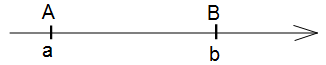
\includegraphics[scale=0.7]{./img/axe1}}
		\end{column}
		\begin{column}{0.465\textwidth}
			\center{\textbf{$AB = a -b $ si $ a > b$} }
			\center{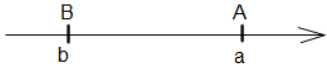
\includegraphics[scale=0.7]{./img/axe2}}
		\end{column}
	\end{columns}
	

	\end{itemize}	
	\end{block}
	
\end{frame}

\begin{frame}
	\frametitle{Distance de deux points}  
	\framesubtitle{Exemple}	
	
	On veut calculer les distances $AB$ et $BC$ :
	\center{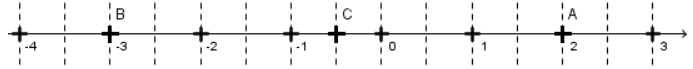
\includegraphics[scale=0.7]{./img/axe3}}\pause

	\begin{exampleblock}{Distance AB}
				
		\begin{itemize}
			\item L'abscisse du point A est +2 et celle du point B est -3.
			\item On a : +2 > -3.
			\item La distance AB est donc égale à la différence entre l'abscisse de A et l'abscisse de B :
			\item[$\Rightarrow $] $AB = (+2) - (-3) = (+2) + (+3) = +5$
		\end{itemize}
	\end{exampleblock}
		
\end{frame}

\begin{frame}
	\frametitle{Distance de deux points}  
	\framesubtitle{Exemple}	
	
	On veut calculer les distances $AB$ et $BC$ :
	\center{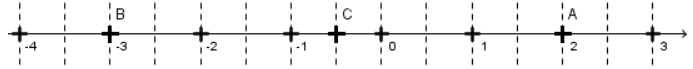
\includegraphics[scale=0.7]{./img/axe3}}
	

	\begin{exampleblock}{Distance BC}
		
		\begin{itemize}
			\item L'abscisse du point B est -3 et celle du point C est -0,5.
			\item On a : -0,5 > -3.
			\item La distance BC est donc égale à la différence entre l'abscisse de C et l'abscisse de B :
			\item[$\Rightarrow $] $BC = (-0,5) - (-3) = (-0,5) + (+3) = +2,5$
		\end{itemize}
	\end{exampleblock}
\end{frame}

\section{Expressions algébriques}

\subsection{Calcul d'une expression algébrique}

\begin{frame}
	\frametitle{Expression algébrique}  
	\framesubtitle{Définition}	
	
	\begin{block}{Définition}
		Une expression algébrique est une suite d'additions et de soustractions de nombres.
	\end{block}
	
	\begin{exampleblock}{Exemple}
		$E = (-3,7) + (-11,9) + (+0,6) - (-11,4) - (+35,8)$\\
		
		$E$ est une expression algébrique.
	\end{exampleblock}
\end{frame}

\begin{frame}
	\frametitle{Expression algébrique}  
	\framesubtitle{Calcul }
	
	\begin{block}{Propriété}
		Pour calculer la \textbf{\underline{somme}} de plusieurs nombres relatifs, on peut \underline{modifier l'ordre des termes} puis les \underline{regrouper} différemment sans que cela ne change le résultat.\pause
	\end{block}	
	
	\begin{block}{Méthode}
		Pour calculer une expression algébrique :
		\begin{itemize}
			\item On commence par \underline{transformer les soustractions en additions}.
			\item On \underline{ajoute les nombres positifs entre eux}. 
			\item On \underline{ajoute les nombres négatifs entre eux}.
			\item On ajoute les deux nombres restants.
		\end{itemize}
	\end{block}
\end{frame}

\begin{frame}[allowframebreaks]
	\frametitle{Expression algébrique}  
	\framesubtitle{Exemple }	
	
	
	\begin{exampleblock}{Exemple 1}
		\begin{itemize}
			\item[$E=$] $(-3,7) + (-11,9) + (+0,6) - (-11,4) - (+35,8)$
			\item[$E=$] $(-3,7) + (-11,9) + (+0,6) \textbf{+ (+11,4) + (-35,8)}$
			\item[$E=$] $\textbf{(+0,6) + (+11,4)} + (-3,7) + (-11,9) + (-35,8)$
			\item[$E=$] $\textbf{(+12)} + (-51,4)$
			\item[$E=$] $ -39,4 $
		\end{itemize}		
	\end{exampleblock}
	
	\begin{exampleblock}{Exemple 2}
		\begin{itemize}
			\item[$F=$] $(-8,5) + (+5,6) - (+2,5) - (-3) + (-4)$
			\item[$F=$] $(-8,5) + (+5,6) \textbf{+ (-2,5) + (+3)} + (-4)$
			\item[$F=$] $ (+5,6) + (+3) + (-8,5) + (-2,5) + (-4)$
			\item[$F=$] $\textbf{(+8,6)} + (-15)$
			\item[$F=$] $ -6,4 $
		\end{itemize}		
	\end{exampleblock}
\end{frame}
	
\subsection{Simplification d'une expression algébrique}

\begin{frame}
	\frametitle{Expression algébrique}  
	\framesubtitle{Simplification }	
	
	\begin{block}{Règle}
		Pour \textbf{\underline{simplifier une expression algébrique}}, on peut :
		\begin{itemize}
			\item Supprimer le signe $\ll$+$\gg$ et les parenthèses des nombres positifs.
			\item \'Ecrire le premier terme sans parenthèse.
		\end{itemize}
	\end{block}
	
	\begin{exampleblock}{Exemples}
		
		\begin{itemize}
			\item $(-8) + (+3) = -8 + 3$
			\item $(-8) + (-3) = (-8) - (+3) = -8 -3 $
			\item $ (+4) - (-7) = (+4) + (+7) = 4 + 7$
			\item $ (+11,5) - (+4,5) = 11,5 - 4,5$ 
		\end{itemize}
	\end{exampleblock}
\end{frame}

\begin{frame}
	\frametitle{Expression algébrique}  
	\framesubtitle{Exemple de calcul d'une expression simplifiée}	
	
	
	\begin{exampleblock}{Exemple}
		\begin{itemize}
			\item[$G=$] $7 + 2,5 - 3,7 + 4,1 - 2,3$
			\item[$G=$] $7 + 2,5 + 4,1 - 3,7 - 2,3$
			\item[$G=$] $(7 + 2,5 + 4,1) - (3,7 + 2,3)$
			\item[$G=$] $13,1 - 6$
			\item[$G=$] $ 7,1 $
		\end{itemize}		
	\end{exampleblock}
	
\end{frame}

\end{document}


\begin{frame}
	\frametitle{}  
	\framesubtitle{}	
	
\end{frame}